\documentclass[11pt,a4paper]{report}

\usepackage[margin=1in]{geometry}
\usepackage[T1]{fontenc}
\usepackage[utf8]{inputenc}
\usepackage{lmodern}
\usepackage{microtype}
\usepackage{graphicx}
\usepackage{booktabs}
\usepackage{array}
\usepackage{longtable}
\usepackage{tabularx}
\usepackage{float}
\usepackage{caption}
\usepackage{hyperref}
\usepackage{fancyvrb}
\usepackage{siunitx}
\usepackage{multirow}
\usepackage{makecell}
\usepackage{threeparttable}
\usepackage{adjustbox}
\usepackage{xurl}

\hypersetup{
  colorlinks=true,
  linkcolor=black,
  urlcolor=blue,
  pageanchor=false
}

\newcolumntype{L}[1]{>{\raggedright\arraybackslash}p{#1}}

\begin{document}

\begin{titlepage}
  \centering
  {\Large King's College London\par}
  \vspace{1.5cm}
  {\Huge \textbf{Appendix and Additional Material}\par}
  \vspace{0.5cm}
  {\Large Improving One-Pixel Attacks on Image Classifiers\par}
  \vspace{1.5cm}

  \begin{tabular}{rl}
    Student name: & Arham Zahid \\
    Student ID: & 22057308 \\
    Programme: & BSc Computer Science \\
    Supervisor: & Hana Chockler \\
  \end{tabular}

  \vfill

  {\large This document accompanies the main report and contains supporting appendix material, supplementary figures and tables, and reproducibility information.\par}

  \vfill
  {\large March 2026\par}
\end{titlepage}

\pagenumbering{roman}
\tableofcontents
\clearpage
\pagenumbering{arabic}
\hypersetup{pageanchor=true}

\appendix

\chapter{Overview}

This appendix accompanies the main report and collects supporting material that would have been
too detailed to include in the report body. Its purpose is to make the submission easier to
inspect, reproduce, and verify.

The appendix has four goals:
\begin{enumerate}
  \item to show how the main report is grounded in a frozen results pack;
  \item to expose supplementary figures and tables not all shown in the report body;
  \item to document the key artefacts present at submission time;
  \item to provide a compact reproducibility route for the submitted implementation.
\end{enumerate}

\chapter{Claims and Evidence Structure}

The main report was written from frozen artefacts rather than from manually copied numbers.
In practice, this means that the quantitative claims in the report are backed by generated CSV,
Markdown summary files, report-ready tables, and report-ready figures stored in the repository.

The evidence chain used for the report can be summarised as follows:

\begin{itemize}
  \item Raw attack outputs are stored as frozen CSV artefacts in \texttt{results/final\_pack/}.
  \item Explanation outputs for the reported 10k runs are stored as frozen CSV artefacts in \texttt{results/final\_pack/}.
  \item Aggregated summaries and comparison narratives are stored as frozen Markdown artefacts in \texttt{results/final\_pack/}.
  \item Report-ready figures are stored in \texttt{report/figures/final\_pack/}.
  \item Report-ready tables are stored in \texttt{report/tables/final\_pack/}.
  \item The report imports these generated assets rather than retyping values by hand.
\end{itemize}

This design was intended to improve traceability and reduce transcription risk.

\section*{Key Frozen Artefacts}

\small
\begin{longtable}{L{0.38\textwidth} L{0.54\textwidth}}
\textbf{Path} & \textbf{Purpose} \\
\hline
\nolinkurl{results/final_pack/CLAIMS_EVIDENCE.md} & Mapping between report claims and supporting artefacts. \\
\nolinkurl{results/final_pack/README.md} & Overview of the frozen results pack and how it is intended to be used. \\
\nolinkurl{results/final_pack/experiments_gpu_10k_overview.md} & High-level summary of the 10k GPU experiment set. \\
\nolinkurl{results/final_pack/story_rq2_guidance_tradeoff.md} & Narrative summary of the guidance trade-off result for RQ2. \\
\nolinkurl{results/final_pack/summary_compare_10000_untargeted_fastprior_rise_guided_gpu_v4.md} & Cross-run comparison summary used to interpret the main RQ2 result. \\
\nolinkurl{results/final_pack/de1px_untargeted_10000.csv} & Frozen untargeted attack results on the 10k index set. \\
\nolinkurl{results/final_pack/de1px_targeted_fastprior_10000.csv} & Frozen fastprior targeted attack results on the 10k index set. \\
\nolinkurl{results/final_pack/before_after_10000_untargeted_gpu.csv} & Frozen explanation metrics for untargeted attack outputs. \\
\nolinkurl{results/final_pack/before_after_10000_fastprior_gpu.csv} & Frozen explanation metrics for fastprior outputs. \\
\nolinkurl{results/final_pack/before_after_10000_rise_guided_gpu.csv} & Frozen explanation metrics for RISE-guided outputs. \\
\nolinkurl{report/figures/final_pack/*} & Report-ready figure assets imported by the main report. \\
\nolinkurl{report/tables/final_pack/*} & Report-ready LaTeX tables imported by the main report. \\
\end{longtable}
\normalsize

\chapter{Artefact Inventory}

The following inventory was generated directly from the repository so that the submitted appendix
records which frozen-pack files and report-ready assets were present at submission time.

{\scriptsize
\VerbatimInput{artefact_inventory.txt}
}

\chapter{Supplementary Figures}

\begin{figure}[H]
  \centering
  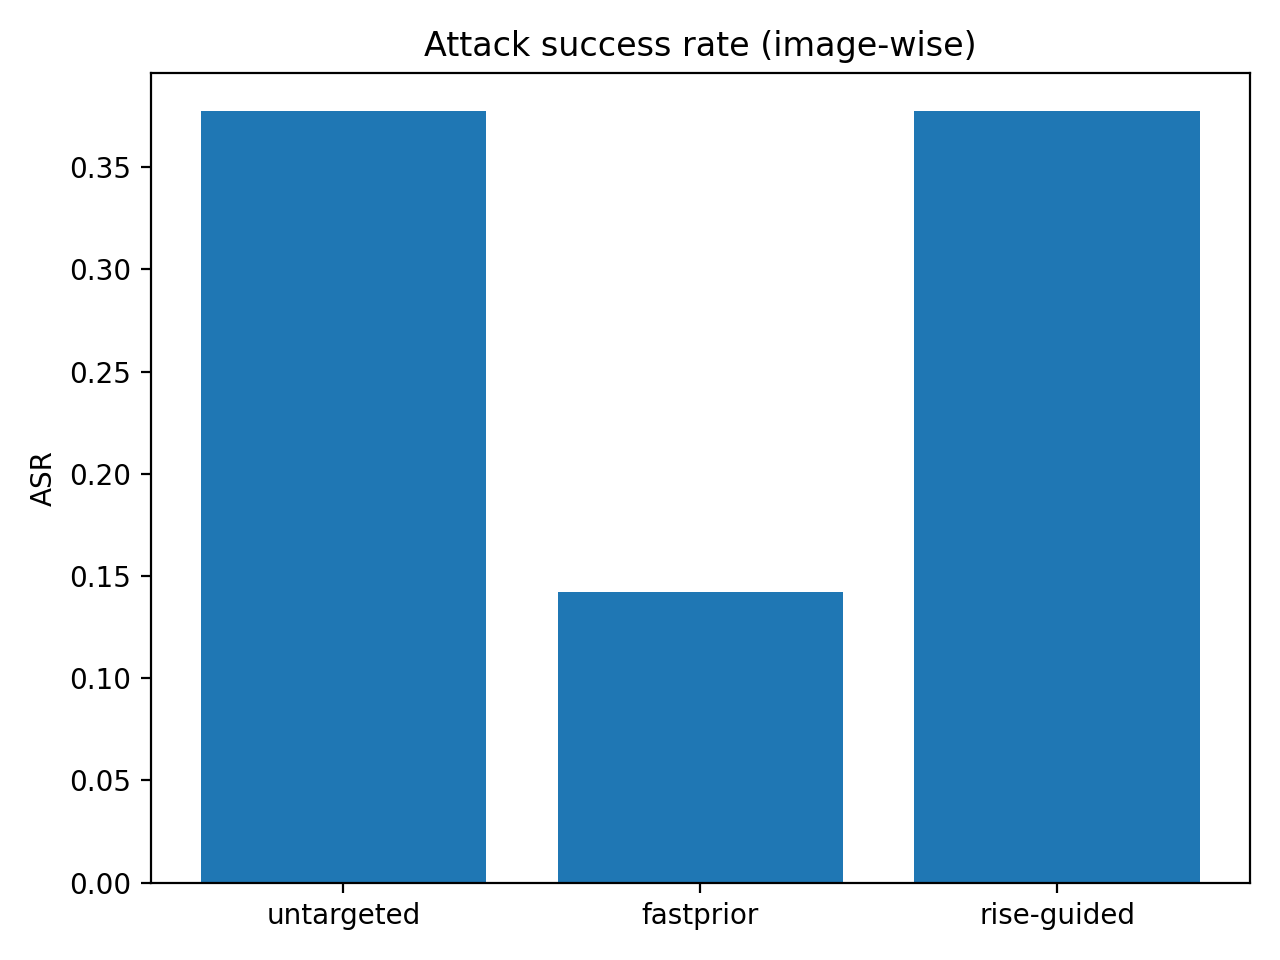
\includegraphics[width=0.92\textwidth]{../report/figures/final_pack/asr_by_run.png}
  \caption{Attack success rate comparison across the reported runs.}
\end{figure}

\begin{figure}[H]
  \centering
  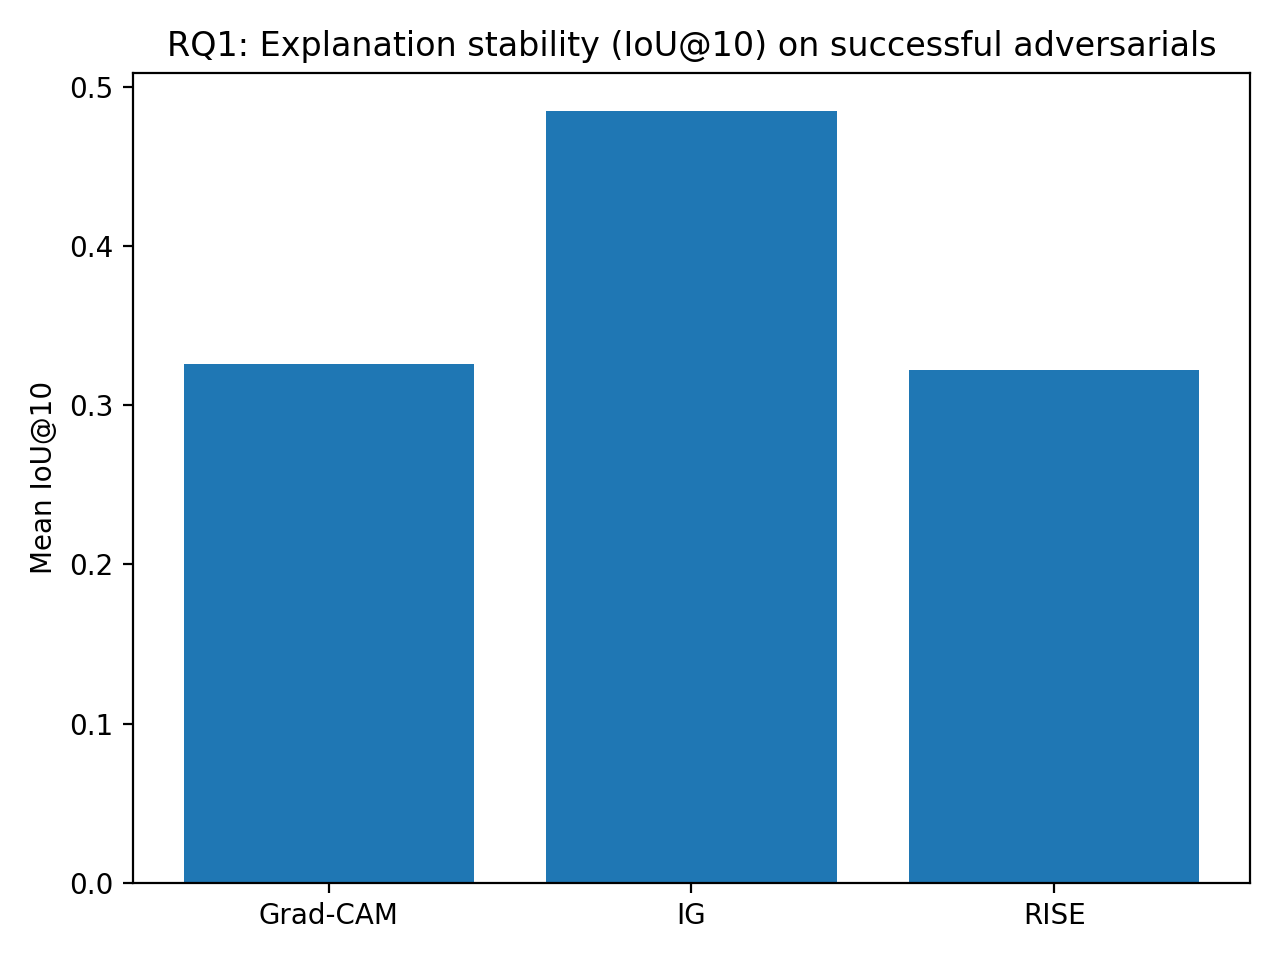
\includegraphics[width=0.92\textwidth]{../report/figures/final_pack/rq1_iou10_adv_mean.png}
  \caption{RQ1 supplementary figure: mean IoU@10 on successful adversarial examples.}
\end{figure}

\begin{figure}[H]
  \centering
  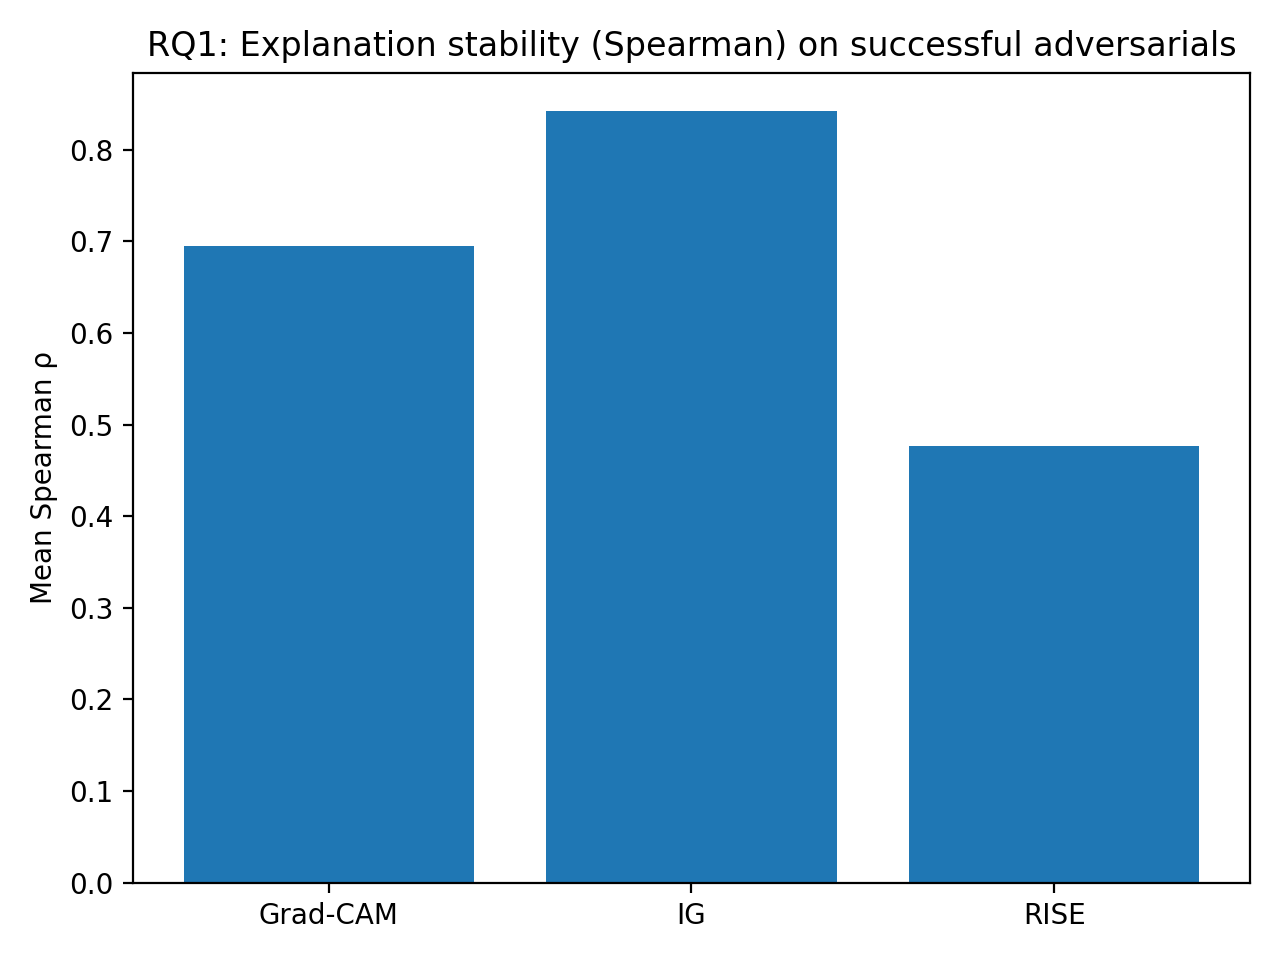
\includegraphics[width=0.92\textwidth]{../report/figures/final_pack/rq1_rho_adv_mean.png}
  \caption{RQ1 supplementary figure: mean Spearman rank correlation on successful adversarial examples.}
\end{figure}

\begin{figure}[H]
  \centering
  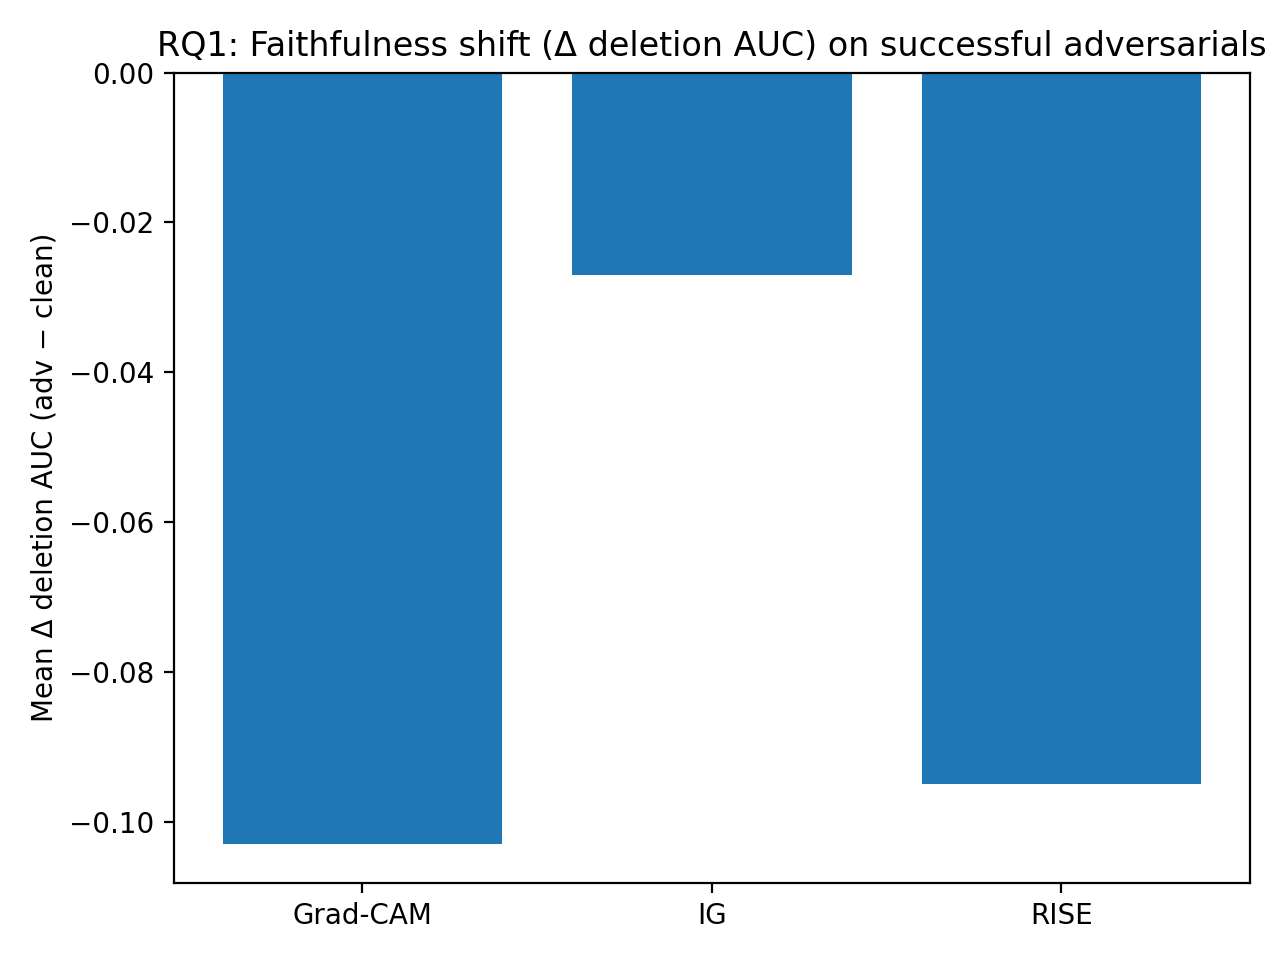
\includegraphics[width=0.92\textwidth]{../report/figures/final_pack/rq1_del_auc_delta_mean.png}
  \caption{RQ1 supplementary figure: mean adversarial-minus-clean deletion AUC change.}
\end{figure}

\begin{figure}[H]
  \centering
  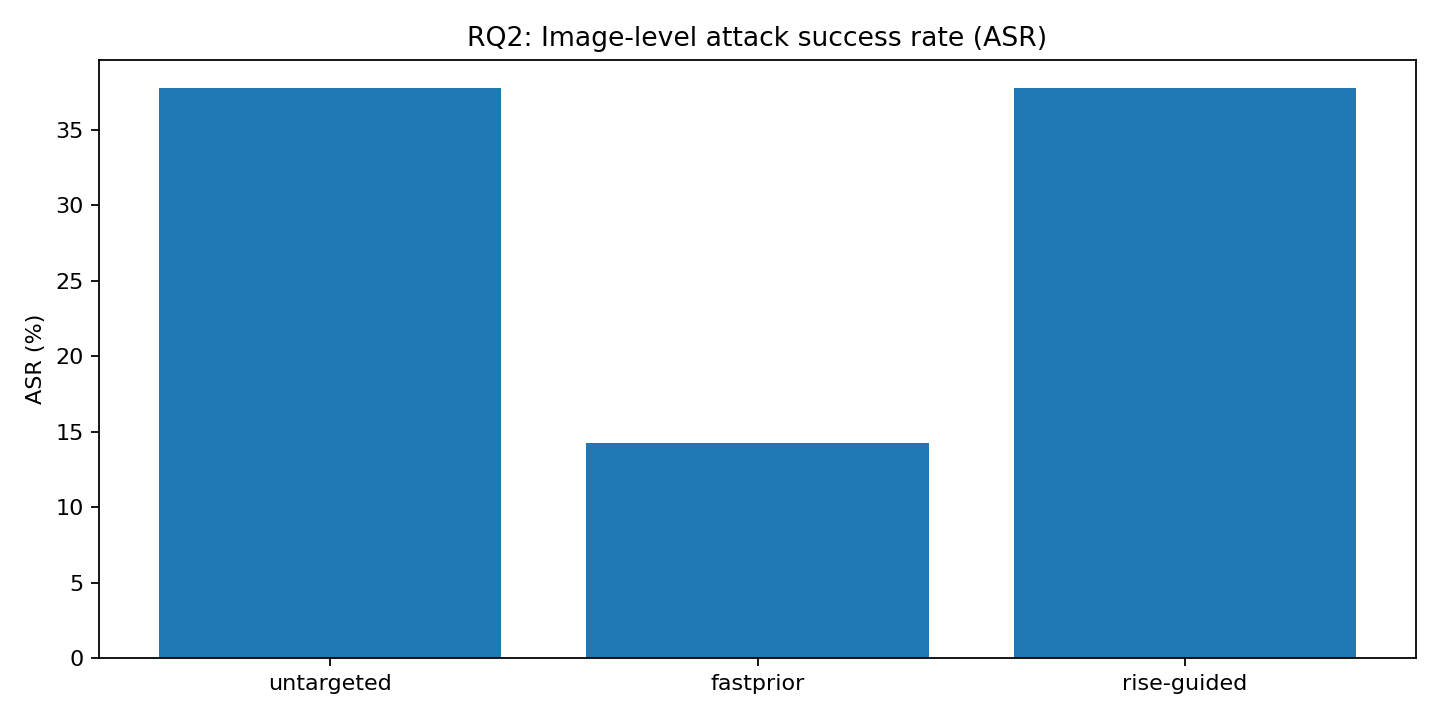
\includegraphics[width=0.92\textwidth]{../report/figures/final_pack/rq2_asr_image_percent.png}
  \caption{RQ2 supplementary figure: image-wise attack success rate by variant.}
\end{figure}

\begin{figure}[H]
  \centering
  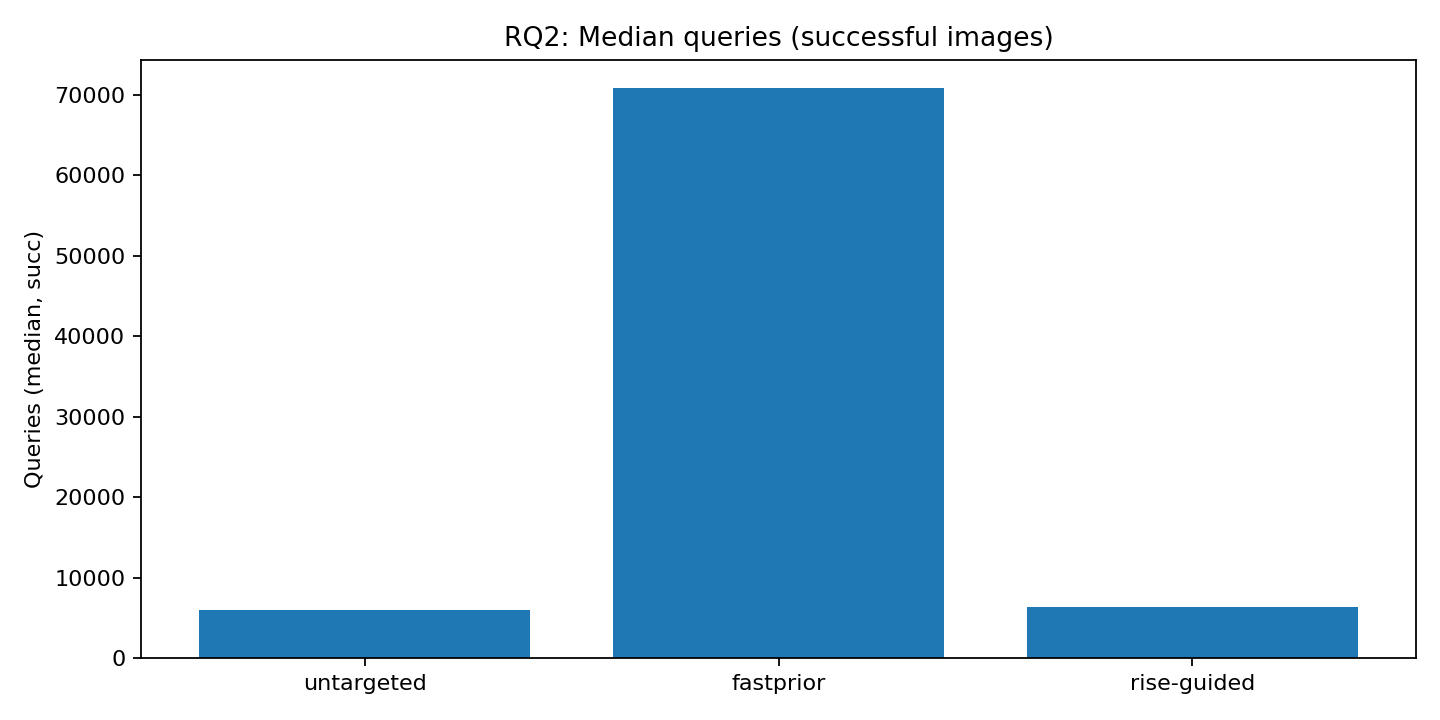
\includegraphics[width=0.92\textwidth]{../report/figures/final_pack/rq2_queries_median_success.png}
  \caption{RQ2 supplementary figure: median successful query cost by variant.}
\end{figure}

\begin{figure}[H]
  \centering
  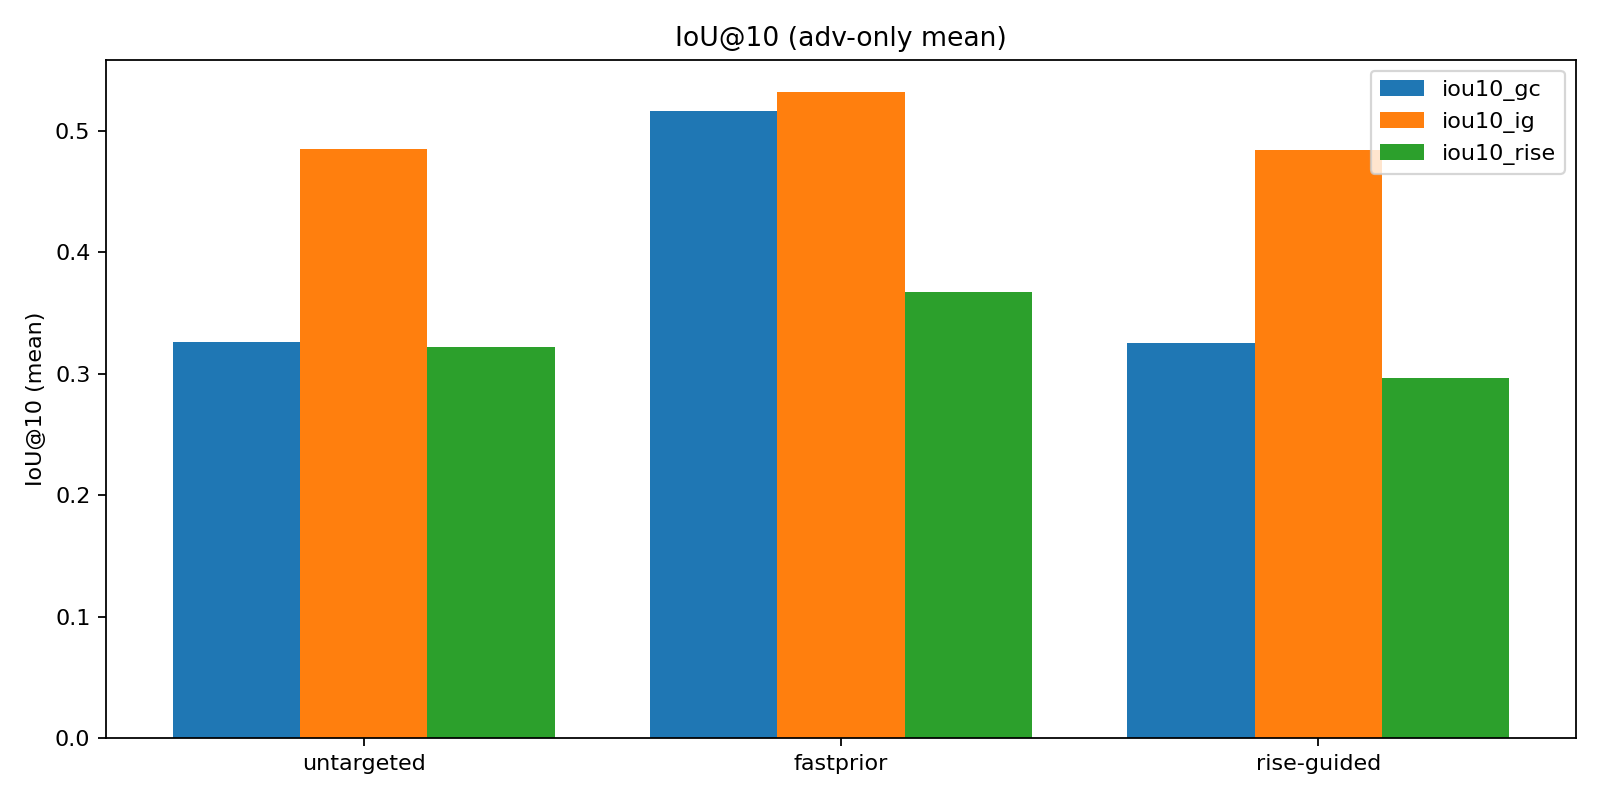
\includegraphics[width=0.92\textwidth]{../report/figures/final_pack/rq2_iou10_adv_mean.png}
  \caption{RQ2 supplementary figure: mean IoU@10 among successful adversarial examples.}
\end{figure}

\begin{figure}[H]
  \centering
  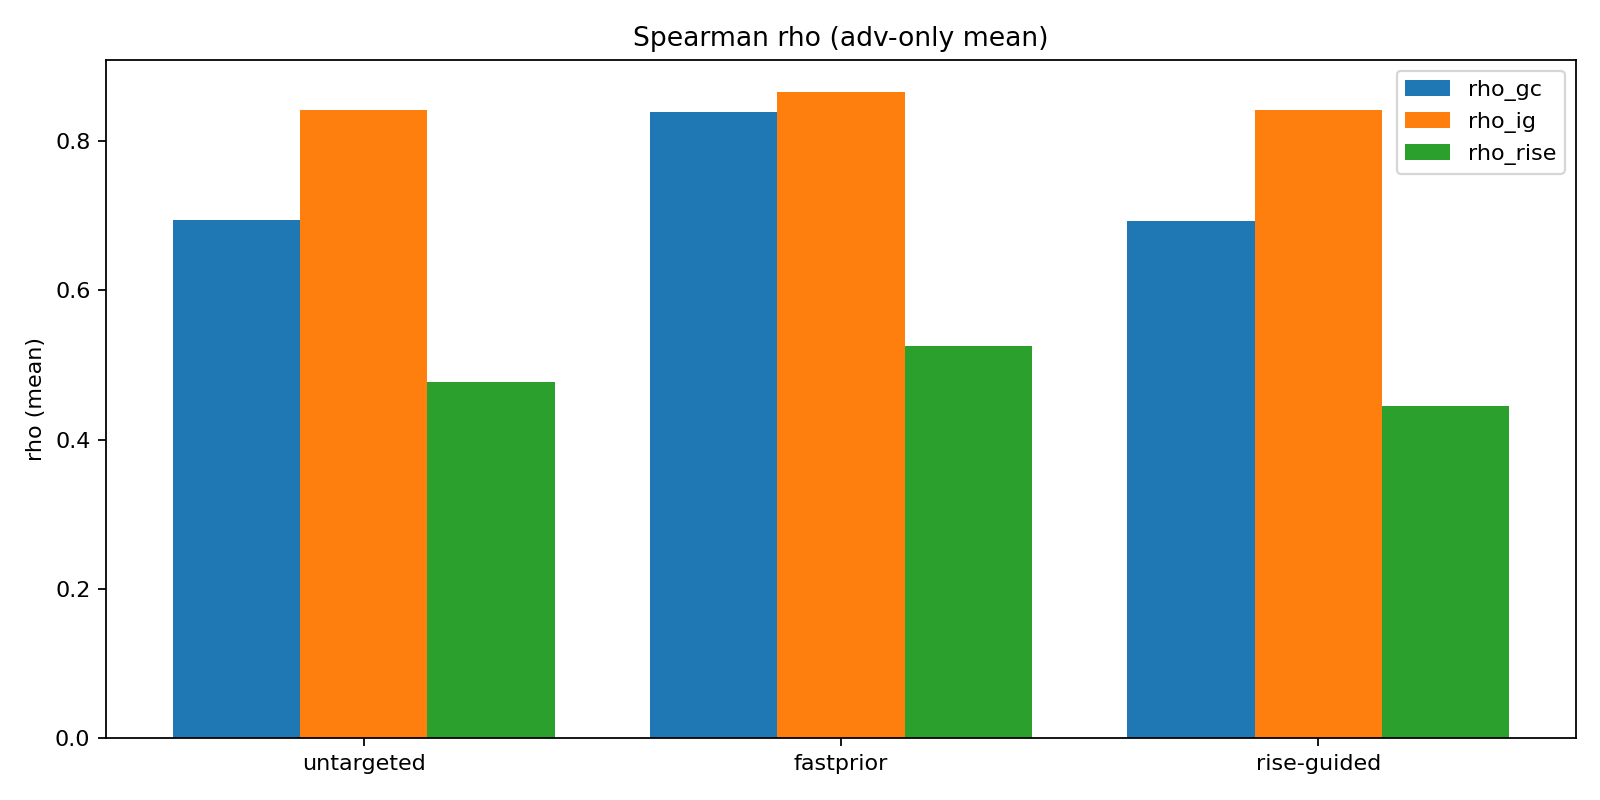
\includegraphics[width=0.92\textwidth]{../report/figures/final_pack/rq2_rho_adv_mean.png}
  \caption{RQ2 supplementary figure: mean Spearman rank correlation among successful adversarial examples.}
\end{figure}

\begin{figure}[H]
  \centering
  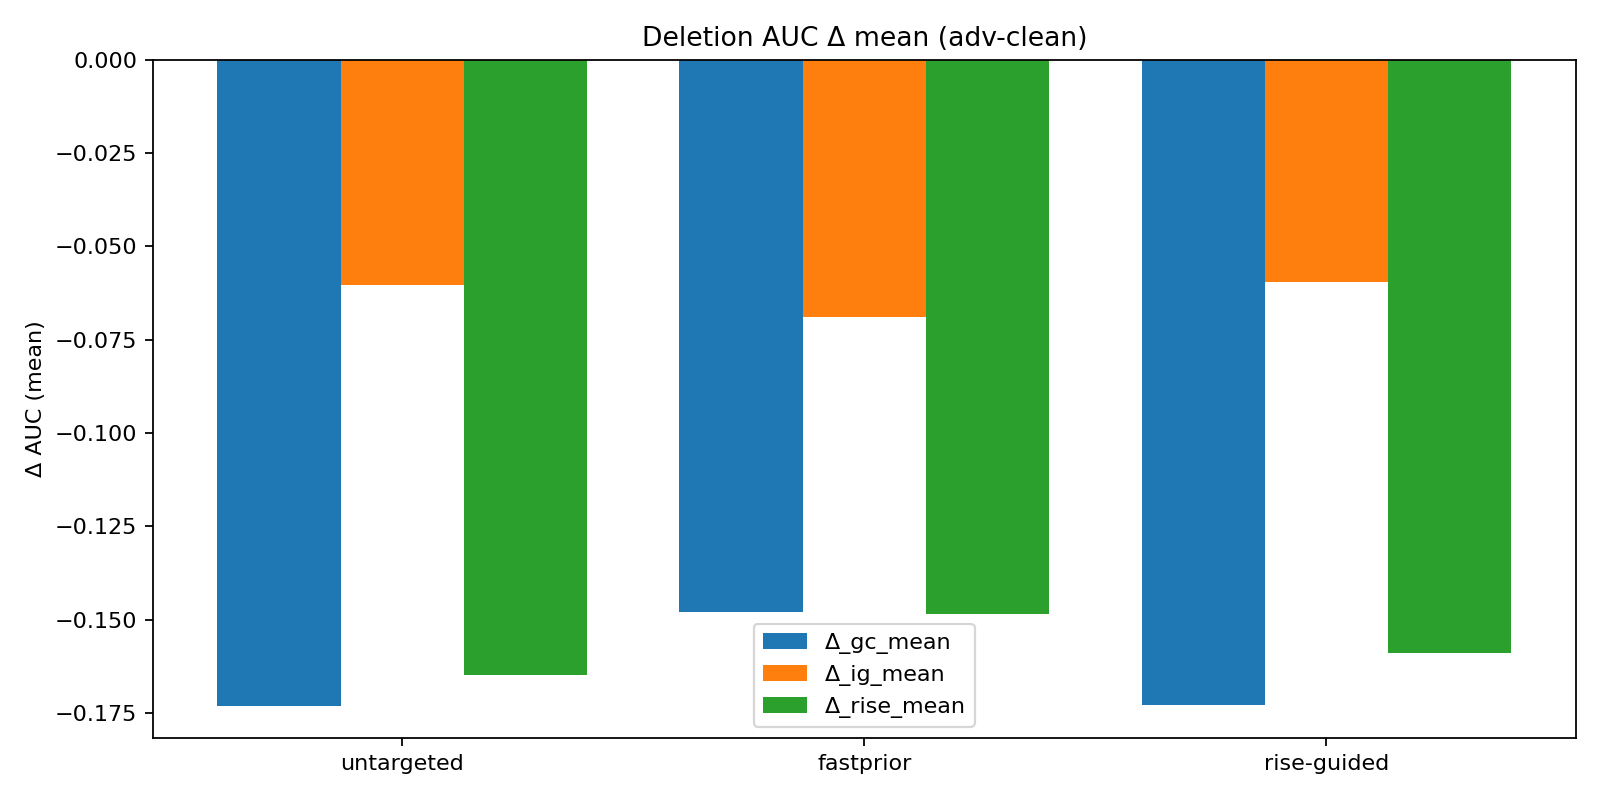
\includegraphics[width=0.92\textwidth]{../report/figures/final_pack/rq2_del_auc_delta_mean.png}
  \caption{RQ2 supplementary figure: mean adversarial-minus-clean deletion AUC change by variant.}
\end{figure}

\clearpage
\chapter{Supplementary Tables}

The following tables are the report-ready exports generated from the frozen results pack.

\begin{table}[t]
\centering
\small
\caption{RQ2 attack outcomes on the eligible CIFAR-10 subset (9{,}213 images): image-wise success rate (ASR) and query cost.}
\label{tab:rq2_attack_summary}
\begin{tabular}{lrrrrr}
\toprule
Run & Eligible & Success & ASR & Median queries (succ) & Median queries (all) \\
\midrule
untargeted & 9,213 & 3,477 & 0.377 & 6,000 & 40,400 \\
fastprior & 9,213 & 1,310 & 0.142 & 70,848 & 70,848 \\
rise-guided & 9,213 & 3,477 & 0.377 & 6,400 & 40,400 \\
\bottomrule
\end{tabular}

\end{table}

\clearpage

\begin{table}
\begingroup
\hbadness=10000
\hfuzz=100pt
\setlength{\emergencystretch}{2em}
\sloppy
[t]
\centering
\scriptsize
\setlength{\tabcolsep}{3pt}
\renewcommand{\arraystretch}{1.15}
\small
\resizebox{0.92\linewidth}{!}{%
\begin{minipage}{\linewidth}
\caption{RQ2 explanation stability on successful adversarial examples (means). Higher IoU@10 and Spearman indicate more stable explanations.}
\label{tab:rq2_stability_means}
\begin{tabular}{lrrrrrr}
\toprule
Run & IoU@10 GC & IoU@10 IG & IoU@10 RISE & Spearman GC & Spearman IG & Spearman RISE \\
\midrule
untargeted & 0.326 & 0.485 & 0.322 & 0.695 & 0.842 & 0.477 \\
fastprior & 0.517 & 0.532 & 0.367 & 0.839 & 0.866 & 0.525 \\
rise-guided & 0.325 & 0.484 & 0.296 & 0.693 & 0.842 & 0.445 \\
\bottomrule
\end{tabular}

\end{minipage}}
\endgroup
\end{table}

\clearpage

\begin{table}[t]
\centering
\small
\setlength{\tabcolsep}{4pt}
\renewcommand{\arraystretch}{1.15}
\caption{RQ2 faithfulness shift under attack: mean change in deletion AUC (adversarial minus clean) on successful adversarial examples. More negative indicates a larger drop.}
\label{tab:rq2_del_delta}
\begin{tabular}{lrrr}
\toprule
Run & $\Delta$DelAUC GC & $\Delta$DelAUC IG & $\Delta$DelAUC RISE \\
\midrule
untargeted & -0.173 & -0.060 & -0.165 \\
fastprior & -0.148 & -0.069 & -0.148 \\
rise-guided & -0.173 & -0.060 & -0.159 \\
\bottomrule
\end{tabular}
\end{table}

\clearpage

\chapter{Reproducibility Route}

This project was structured so that the submitted PDFs could be rebuilt from version-controlled
sources and imported generated assets.

A compact local route is:

\begin{Verbatim}[fontsize=\small]
cd ~/Projects/kcl-6ccs3prj-2025
python3 -m venv .venv
source .venv/bin/activate
pip install -r requirements.txt

# Rebuild the main report PDF
cd report
latexmk -pdf -halt-on-error main.tex

# Rebuild the appendix PDF
cd ../appendix
latexmk -pdf -halt-on-error main.tex
\end{Verbatim}

Under the current project setup, the main report is produced at
\path{report/build/main.pdf} and the appendix is produced at
\path{appendix/main.pdf}.

The main report uses generated figure and table assets stored under
\path{report/figures/final_pack/} and
\path{report/tables/final_pack/}.
The appendix inventory and the frozen-pack structure are included so that a marker can inspect
the evidence trail without having to search through the repository manually.

\chapter{Why this Appendix Exists}

The main report was intentionally kept concise. This appendix therefore serves as a supporting
document that makes the submission more transparent and easier to audit. It highlights the
submission's evidence trail, preserves the frozen artefact inventory, and surfaces additional
figures and tables that strengthen the case for reproducibility and careful experimental method.

\end{document}
